\section{Architectural Design}
\subsection{Overview: high-level components and interactions}
\begin{figure}[H]
    \begin{center}
        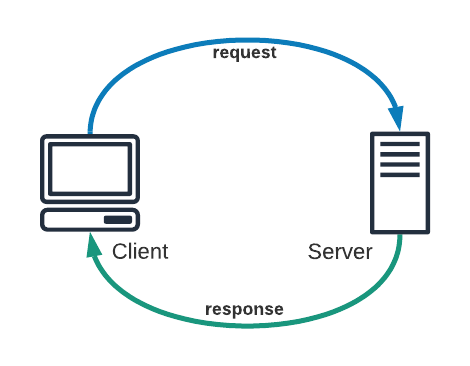
\includegraphics[width=\textwidth/2]{img/Client-Server.png}
        \caption{Client-Server paradigm}\label{client_server_par}
    \end{center}
\end{figure}

As figure \ref{client_server_par} represents, the system is a distributed application which follows the common known client-server paradigm.

In particular, there are two different types of client, which makes it either thin and fat at the same time.

The first one is a \textit{Web Browser}, which is by definition a thin client, because of its total dependency from the server.
This type of client does not contain the application business logic, but only the presentation layer.

The second one, instead, is a mobile application, which contains an internal database in order to make it less dependent from the server. This aspect makes it a more thick client.

In both cases the server is \textit{fat} and contains all the data management and business logic.

In this section the architecture will be described in an easy way, justifying all the choices for adopted patterns.

\begin{figure}[H]
    \begin{center}
        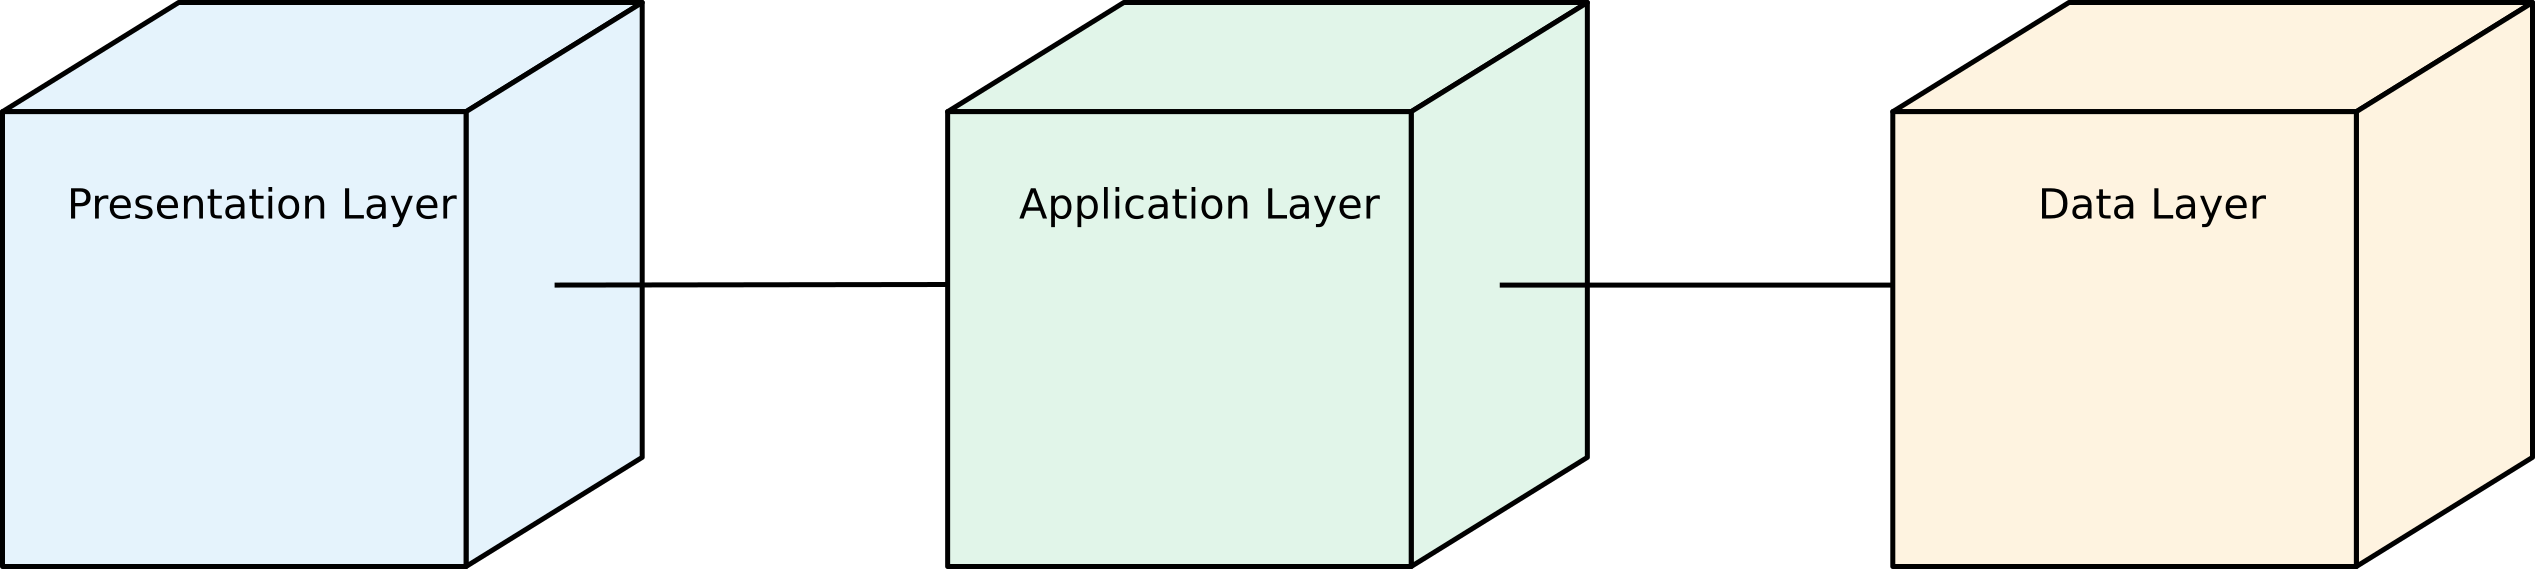
\includegraphics[width=\textwidth]{img/3-tier.png}
        \caption{Three layers application}\label{three_tier_desc}
    \end{center}
\end{figure}

In figure\ref{three_tier_desc} the three S2B layers are shown, which respectively are:
\begin{itemize}
    \item \textbf{Presentation Layer:} it manages the presentation logic and, consequently, all the interactions with the end user. This is also called \textit{rendering layer}.
    \item \textbf{Application (Logic) Layer:} it manages the business functions that the S2B must provide.
    \item \textbf{Data Layer:} it manages the safe storage and the relative access to data.
\end{itemize}

As shown in the high level representation of figure \ref{three_tier_application} the S2B is divided into three layers that are physically separated by installing them on different tiers. A tier is a physical (or a set of) machine, each of them with its own computational power.

The application described in this document is composed by four tiers.

%\begin{figure}[H]
%    \includegraphics[width=\textwidth]{img/}
%    \caption{Architecture of the application}\label{three_tier_application}
%\end{figure}     Mettere immagine 


\subsection{Component view}
\subsection{Deployment view}

\begin{figure}[H]
    \begin{center}
        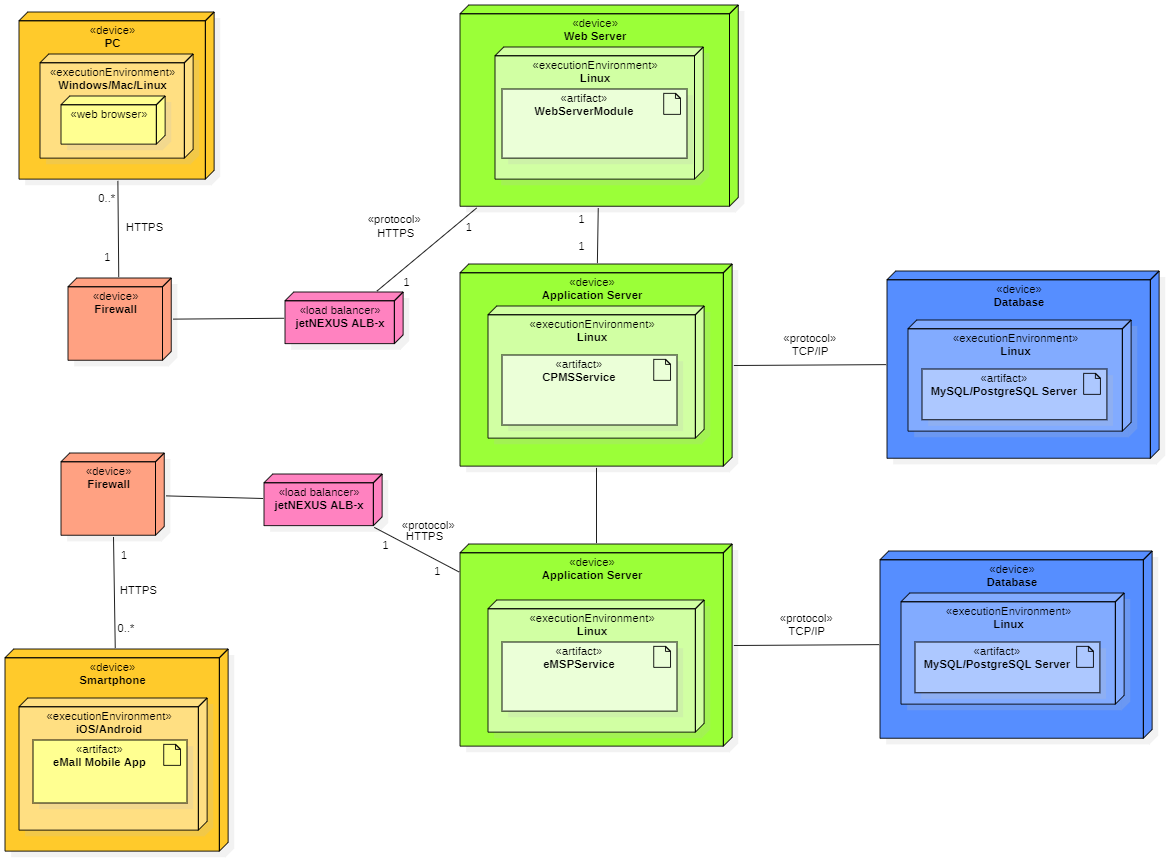
\includegraphics[width=\textwidth]{img/DeploymentDiagram.PNG}
        \caption{Deployment Diagram}\label{deployment_diagram}
    \end{center}
\end{figure}

The deployment diagram in figure\ref{deployment_diagram} shows the needed components for a correct system behavior and the protocols to communicate. As shown in the above image, firewalls and load balancers manage the data stream
from the devices to the servers. First of all, firewalls are in charge of filtering packets
received from the Internet. Then, the packets pass through the load balancer, where
the workload is distributed among the available resources to increase capacity and
reliability.
Each device has its own Operating System where the software runs.
The tiers in the image are the following:
\begin{itemize}
    \item \textbf{Tier 1:} it is the client machine, which can be a computer with a web browser (running, for example, on Windows 10 OS) or the downloadable mobile application (available on both Apple's store and Google's Store).
    \item \textbf{Tier 2:} it includes the replicated web servers, which do not execute any business logic, but simply receive requests from the client, route them to the application servers and serve an HTML file fo the client, which will build the page thanks to client-side scripting. They also append the styling logic of the page (CSS sheets, JS sheets, etc.).
    \item \textbf{Tier 3:} it contains the application servers, which run the core functionalities of the S2B. The whole application layer is mapped into this tier, which communicates to the client tier through APIs, which will be used from the web servers (in case of webapp) and the native application (in case of mobile app download). Furthermore, it communicates to the data tier through the DBMS gateway.
    \item \textbf{Tier 4:} it is composed by the DBMS servers. They store the data and execute actions on it, according to the instruction given by the application servers.
\end{itemize}
\subsection{Runtime view}
\subsection{Component interface}
\subsection{Selected architectural styles and patterns}
\subsection{Other design decisions}

